\section{Evaluation}%
\label{sec:evaluation}
\subsection{Graphs of Loss over Time}%
\label{sub:graphs_of_loss_over_time}
\begin{figure}[htpb]
    \centering
    % This file was created by tikzplotlib v0.9.1.
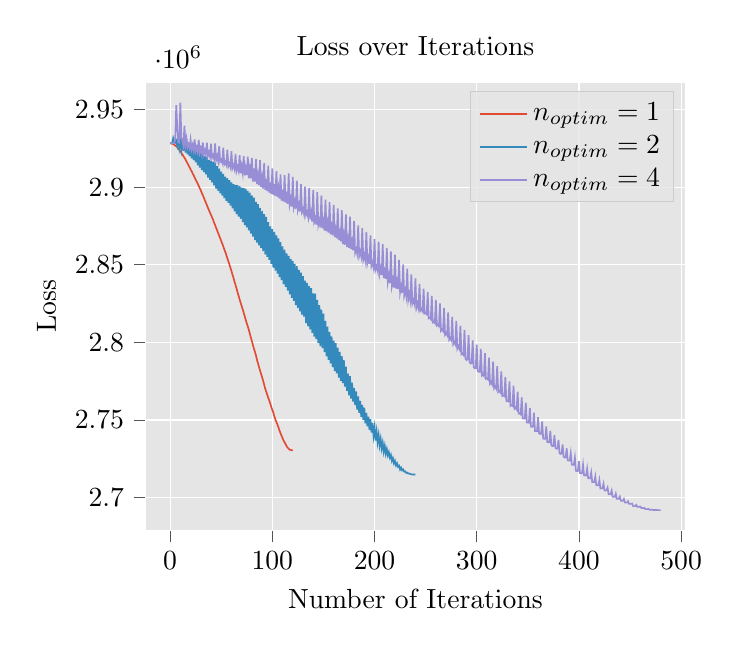
\begin{tikzpicture}

\definecolor{color0}{rgb}{0.886274509803922,0.290196078431373,0.2}
\definecolor{color1}{rgb}{0.203921568627451,0.541176470588235,0.741176470588235}
\definecolor{color2}{rgb}{0.596078431372549,0.556862745098039,0.835294117647059}

\begin{axis}[
axis background/.style={fill=white!89.8039215686275!black},
axis line style={white},
legend cell align={left},
legend style={fill opacity=0.8, draw opacity=1, text opacity=1, draw=white!80!black, fill=white!89.8039215686275!black},
tick align=outside,
tick pos=left,
title={Loss over Iterations},
x grid style={white},
xlabel={Number of Iterations},
xlabel near ticks,
xmajorgrids,
xmin=-24, xmax=504,
xtick style={color=white!33.3333333333333!black},
y grid style={white},
ylabel={Loss},
ylabel near ticks,
ymajorgrids,
ymin=2678750.65, ymax=2967662.35,
ytick style={color=white!33.3333333333333!black}
]
\addplot [semithick, color0]
table {%
0 2928199.75
1 2928404
2 2928023.75
3 2927797.5
4 2927321.5
5 2926868
6 2926325
7 2925731.5
8 2924925.5
9 2924131.75
10 2923069.5
11 2922090
12 2921113.75
13 2920027
14 2918980.5
15 2917948.25
16 2916506.5
17 2915388.75
18 2914115.25
19 2912909.5
20 2911492
21 2910323.5
22 2908867.75
23 2907734
24 2906225.75
25 2904845.75
26 2903565.25
27 2902217.5
28 2900836.25
29 2899333
30 2897946.75
31 2896240.25
32 2894805
33 2893268.75
34 2891548
35 2890055
36 2888339.75
37 2886707.5
38 2885186.75
39 2883617.5
40 2882139
41 2880556.5
42 2879082.75
43 2877150
44 2875578.5
45 2873761.5
46 2872139
47 2870368.5
48 2868740.75
49 2867025.5
50 2865359.75
51 2863667.75
52 2861915.5
53 2859946.25
54 2858182
55 2856216
56 2854191
57 2852193.75
58 2850183.75
59 2848045.5
60 2845995.5
61 2843666.5
62 2841579.5
63 2839096
64 2836941.75
65 2834595.75
66 2832214.5
67 2829967
68 2827663.25
69 2825525
70 2823362.5
71 2821345
72 2819041.25
73 2816824.75
74 2814539.75
75 2812260.5
76 2810274.25
77 2808043.5
78 2805545.75
79 2803052.5
80 2800767.25
81 2798293.5
82 2795985.25
83 2793832.5
84 2791595
85 2788672
86 2786485.25
87 2784024.25
88 2781863.5
89 2779719.75
90 2777457
91 2775303
92 2772732
93 2770243.25
94 2768257.75
95 2766231.5
96 2764311.75
97 2762489.5
98 2760540.25
99 2758260.25
100 2756408
101 2754677.5
102 2752294.5
103 2750273.75
104 2748613
105 2747069.25
106 2745134.25
107 2743260.5
108 2741409.5
109 2739913.75
110 2738261.25
111 2736697.75
112 2735572.75
113 2734396.5
114 2733080
115 2732164
116 2731501.5
117 2730859.5
118 2730700
119 2730492.5
120 2730407
};
\addlegendentry{$n_{optim}=1$}
\addplot [semithick, color1]
table {%
0 2928199.75
2 2928404
3 2931519
4 2928987.25
5 2928645
6 2929930.5
7 2926775.5
8 2931293.75
9 2925490.5
10 2930543.5
11 2924449.75
12 2930835
13 2923475.5
14 2931939.25
15 2922362
16 2931025.75
17 2921118
18 2928871.75
19 2919988.25
20 2928103
21 2918672.25
22 2927102.25
23 2917424.5
24 2926587
25 2915999.5
26 2927003
27 2914159
28 2924906
29 2912562
30 2924253.75
31 2911044
32 2921953.25
33 2909790.5
34 2920049
35 2908221.25
36 2919286.75
37 2906234.25
38 2917540
39 2904676.5
40 2916767
41 2903086.75
42 2916491.5
43 2901120.75
44 2915810.5
45 2899036
46 2913616.5
47 2897707.75
48 2911878
49 2896111.25
50 2910008.25
51 2894524
52 2908617.5
53 2892952.75
54 2906777
55 2891192.5
56 2905749.25
57 2889901.5
58 2904582.25
59 2888088
60 2903075.5
61 2886373.25
62 2901874.5
63 2884351.25
64 2901402.5
65 2882581.5
66 2901359
67 2881082.5
68 2900741.5
69 2879610.5
70 2899731
71 2877566.5
72 2899359.5
73 2875505.5
74 2898907.25
75 2874126.75
76 2897538.25
77 2872198.25
78 2896515.5
79 2870057.5
80 2894720.5
81 2868101.5
82 2893233
83 2865967.5
84 2890467
85 2864323
86 2889132.25
87 2862450.5
88 2886680.75
89 2860857
90 2884645.5
91 2858794
92 2882601.5
93 2856653.25
94 2880847.5
95 2855025.25
96 2877403.75
97 2853157.75
98 2874731
99 2850528.25
100 2873004.25
101 2848100
102 2871149
103 2846263.5
104 2868981.5
105 2844354.5
106 2866995.75
107 2842044.25
108 2864535.75
109 2840162.5
110 2861853
111 2837510.75
112 2859682
113 2835717
114 2857278.5
115 2833344.75
116 2855646
117 2830923.5
118 2853727.25
119 2828692
120 2852447.25
121 2826683
122 2850485.25
123 2823932
124 2849178.5
125 2822127.25
126 2846655.5
127 2820045
128 2844900.5
129 2817935.25
130 2842622.75
131 2816559.25
132 2839763
133 2812461.25
134 2838253.5
135 2810270.5
136 2836413.5
137 2808169.5
138 2834982
139 2806103.75
140 2831624
141 2803774
142 2831382.5
143 2802169
144 2827287.75
145 2799667
146 2823947.75
147 2797504
148 2821033.75
149 2796238
150 2818446.25
151 2793647.5
152 2813790.75
153 2791013.25
154 2810187.75
155 2788703
156 2806540.25
157 2786470.5
158 2803756.5
159 2783988.5
160 2801152.25
161 2781528
162 2799443
163 2779953.75
164 2796644.25
165 2777275.5
166 2793832
167 2775127.75
168 2791092.5
169 2773679.5
170 2788460.5
171 2771453.5
172 2784304.75
173 2768763.25
174 2779820.25
175 2765796.25
176 2778206
177 2763765
178 2774016.5
179 2761771.5
180 2770609.25
181 2759569.75
182 2768387.5
183 2756717.5
184 2765150.25
185 2754608.5
186 2762251.5
187 2752021
188 2759704.5
189 2750076.25
190 2757905
191 2747848.25
192 2754512.25
193 2745837
194 2752072
195 2743713.25
196 2750498.5
197 2741844
198 2747916
199 2739849
200 2745090.75
201 2736670.5
202 2742516.5
203 2735622.5
204 2740326.25
205 2733613.75
206 2737803.5
207 2731635.5
208 2735336.75
209 2729558
210 2733270.75
211 2728189.75
212 2731222.5
213 2727192.75
214 2729276
215 2725749
216 2727440.5
217 2723585.75
218 2725349
219 2722034
220 2723622
221 2720693.25
222 2722018.5
223 2719789
224 2720498.75
225 2718040.75
226 2719267.75
227 2717526
228 2718120.5
229 2716679
230 2716862.5
231 2715850.75
232 2716050.25
233 2715426.75
234 2715453.25
235 2715121
236 2714998
237 2714824
238 2714798
239 2714841.5
240 2714810
};
\addlegendentry{$n_{optim}=2$}
\addplot [semithick, color2]
table {%
0 2928199.75
4 2928404
5 2931519
6 2952907
7 2938537.75
8 2928986.75
9 2928646
10 2954530
11 2932171
12 2929930.5
13 2926776
14 2939597
15 2927209
16 2931293.5
17 2925490.5
18 2927376.75
19 2925068
20 2930543.25
21 2924450.5
22 2927242.5
23 2923913.75
24 2930835
25 2923473.5
26 2925768
27 2922789.25
28 2930506.5
29 2922376
30 2924988.5
31 2921691.25
32 2928816.75
33 2921354
34 2923756
35 2920954.75
36 2928597
37 2920221
38 2922395.5
39 2919615.5
40 2928038.75
41 2918981
42 2920494
43 2918200.25
44 2928236
45 2917448
46 2920025.5
47 2916677.75
48 2926469
49 2916386.25
50 2917568.75
51 2915815.75
52 2925393.5
53 2914726.75
54 2916173.5
55 2914369
56 2924230
57 2913501.25
58 2915132
59 2912932.5
60 2923135.5
61 2912217.75
62 2914158.5
63 2911689.5
64 2921458.75
65 2910669.5
66 2913210
67 2910531.5
68 2920603
69 2908900.25
70 2913645.75
71 2909147
72 2919982
73 2907586
74 2912421.5
75 2907763.25
76 2919715.5
77 2905706.75
78 2911906
79 2905677.75
80 2918806.5
81 2903669.5
82 2912048.5
83 2903552.75
84 2918016.25
85 2902055.75
86 2907668.5
87 2901272.5
88 2917336
89 2900050.25
90 2905910
91 2899088.25
92 2915487.25
93 2898297
94 2905224.5
95 2897470.25
96 2913853.75
97 2896565.25
98 2903111.5
99 2895768
100 2912152.5
101 2895109.5
102 2901898
103 2894303.5
104 2910337.5
105 2893626.5
106 2899546.5
107 2892726.5
108 2908181.25
109 2891427.5
110 2898370
111 2890788
112 2907922
113 2890033
114 2897164.5
115 2889219
116 2908881
117 2888971.75
118 2892578
119 2887469.25
120 2906632.5
121 2887316.5
122 2890451.75
123 2885973
124 2904141.5
125 2885622.5
126 2888718
127 2884373.5
128 2902026.5
129 2884073.5
130 2885814
131 2882702.5
132 2900331.75
133 2882194
134 2883981
135 2880874.25
136 2899460.5
137 2879300
138 2883405.5
139 2877880.5
140 2898144.5
141 2877653.5
142 2879902.25
143 2875960.25
144 2896837
145 2875737.25
146 2878503.5
147 2873941.5
148 2894726
149 2873546.5
150 2877883
151 2872106.5
152 2892016.75
153 2871538.5
154 2876845.5
155 2870733.75
156 2890366
157 2869685.75
158 2874251.25
159 2868938.5
160 2888545.5
161 2867879.5
162 2872484.5
163 2867112.5
164 2886311.75
165 2865912.25
166 2870286.25
167 2865167.75
168 2885211
169 2863254.25
170 2869073
171 2862936.5
172 2882472
173 2861403.25
174 2866408
175 2860875
176 2881003.75
177 2860097.25
178 2864477.5
179 2859404.25
180 2878322
181 2857769.75
182 2859902.75
183 2857196.25
184 2875419.5
185 2855674.5
186 2858157
187 2855239.25
188 2873535.5
189 2853360
190 2856233.5
191 2852787.75
192 2871132.25
193 2851252
194 2854454.75
195 2850475
196 2868894.5
197 2849330
198 2851386.25
199 2848227.75
200 2866514
201 2846905
202 2848851
203 2846198
204 2864965.5
205 2844239.75
206 2847604.25
207 2843407.5
208 2863290
209 2841462.5
210 2845406.25
211 2840944.25
212 2860815
213 2839086.75
214 2842887
215 2838130.5
216 2858655.25
217 2836468
218 2840247
219 2835368.5
220 2856573.75
221 2834742
222 2839022.75
223 2834323.25
224 2853074.5
225 2832229
226 2835825.5
227 2831837
228 2850185.75
229 2830401.5
230 2833704
231 2829922.5
232 2847479.5
233 2827490.75
234 2831030
235 2827197
236 2843775.5
237 2825094
238 2827174.75
239 2824745.5
240 2841162.5
241 2822278.75
242 2824818
243 2821983.25
244 2837656
245 2820441.25
246 2821424
247 2820087.5
248 2834584.75
249 2818584.5
250 2818887.25
251 2818107.75
252 2832313
253 2815553.25
254 2816023
255 2815078.75
256 2829912
257 2812889.5
258 2813376.5
259 2812419.25
260 2827328.75
261 2810775.75
262 2811369.75
263 2810414.25
264 2825170.5
265 2807493.75
266 2808363.75
267 2807343.25
268 2822183
269 2804852.5
270 2805995.5
271 2804687
272 2819245.5
273 2801714.5
274 2802770.5
275 2801541
276 2816338.5
277 2798895.5
278 2800155.5
279 2798742.75
280 2813754.5
281 2795917
282 2797501.25
283 2795896.25
284 2810685.5
285 2792306.5
286 2792800
287 2791871.5
288 2807961.5
289 2789456
290 2788589.5
291 2789207
292 2804639.5
293 2787161.25
294 2786358.5
295 2786564
296 2801227
297 2783960
298 2783325.25
299 2783408.25
300 2798569.5
301 2781562
302 2781036
303 2781059.75
304 2795805.5
305 2778705.75
306 2779507.5
307 2778376.75
308 2792963.5
309 2776519
310 2776781.75
311 2776041
312 2790200.5
313 2773316.25
314 2774441.25
315 2773055.25
316 2787563.75
317 2770444.25
318 2771586.5
319 2770269.5
320 2784672.5
321 2768076.75
322 2768762.25
323 2767814.75
324 2781309.25
325 2765488.5
326 2765645.25
327 2765246
328 2777676.75
329 2762150
330 2762298.5
331 2761950.25
332 2774877
333 2759084.5
334 2759626.5
335 2759051
336 2772058
337 2757250
338 2757830
339 2756812
340 2768231.5
341 2754099
342 2754194.5
343 2753593.75
344 2764597.5
345 2751011.75
346 2750922.75
347 2750925.25
348 2761208.5
349 2748327
350 2748295
351 2748240.5
352 2757711
353 2745724.5
354 2745656
355 2745676.5
356 2754674
357 2742775
358 2742849
359 2742841.25
360 2751816.25
361 2741277
362 2740996
363 2741054
364 2749013
365 2737999
366 2737857.75
367 2737876
368 2745745.25
369 2735794.75
370 2735559.75
371 2735571
372 2742873
373 2733601.5
374 2733132
375 2733264
376 2740098.75
377 2731908.75
378 2731480.5
379 2731608
380 2737095.5
381 2728558.75
382 2728105
383 2728277.75
384 2734261.75
385 2726138.25
386 2725813
387 2725935
388 2731711.5
389 2723964
390 2723776.75
391 2723811.5
392 2728608
393 2721219.5
394 2721023.25
395 2721049.5
396 2725801.75
397 2717226.5
398 2717088.5
399 2717142.75
400 2723451.5
401 2715773.5
402 2715684
403 2715722
404 2721099.75
405 2714332.5
406 2714194.25
407 2714254
408 2718602.5
409 2712458.5
410 2712344
411 2712384
412 2716144.5
413 2709978.25
414 2709957
415 2709946.5
416 2713565.5
417 2707832.5
418 2707854.5
419 2707836.75
420 2711317.5
421 2705792.5
422 2705932.25
423 2705891.25
424 2708864.5
425 2704525.25
426 2704626
427 2704614.5
428 2706393
429 2702181.5
430 2702065
431 2702082.25
432 2704443
433 2700543.75
434 2700524
435 2700533
436 2702512.5
437 2699248.5
438 2699211
439 2699217
440 2700596.25
441 2697963.25
442 2697910
443 2697909.5
444 2699125.75
445 2696756.5
446 2696746
447 2696746.5
448 2697615.25
449 2695918.5
450 2695913.5
451 2695912.75
452 2696108.25
453 2694491.5
454 2694473.75
455 2694474.5
456 2695258.25
457 2694101.75
458 2694092.5
459 2694092
460 2694236
461 2693216.5
462 2693206.75
463 2693207.5
464 2693354.5
465 2692561
466 2692560.5
467 2692560.25
468 2692609
469 2692121
470 2692127.25
471 2692129
472 2692138.75
473 2691948
474 2691948.25
475 2691948.75
476 2691983
477 2691883
478 2691883
480 2691883
};
\addlegendentry{$n_{optim}=4$}
\end{axis}

\end{tikzpicture}

    \caption{Loss over number of gradient descent iterations for $N=11$ for various $n_{optim}$, and $n=5$. \emph{Lower bound constant has not been subtracted yet.}}
    \label{fig:11_curves}
\end{figure}

\autoref{fig:11_curves} shows the loss over time for $N=11$ for various $n_{optim}$ with $n=5$ (number of RAS iterations). All of the tested values of $N$ from $[6,30]$ had similar curves. The sharp discontinuities within the curves when $n_{optim}>1$ are attributed to the reinitialization of $S$, after revealing each of the $N^2$ tokens. Furthermore, it can be observed that a higher $n_{optim}$ leads to a lower final loss.

\subsection{Comparison to State of the Art}%
\label{sub:comparison_to_state_of_the_art}

\begingroup
\renewcommand{\arraystretch}{0.7}
\begin{table}[htpb]
\begin{center}
\begin{tabular}{r|l}
  $N$ & Loss\\\hline
  6&\num{5\,526}\\
  7&\num{17\,779}\\
  8&\num{57\,152}\\
  9&\num{144\,459}\\
  10&\num{362\,950}\\
  11&\num{740\,798}\\
  12&\num{1\,585\,264}\\
  13&\num{2\,888\,120}\\
\end{tabular}
\begin{tabular}{r|l}
  $N$ & Loss\\\hline
  14&\num{5\,457\,848}\\
  15&\num{9\,164\,700}\\
  16&\num{15\,891\,088}\\
  17&\num{25\,152\,826}\\
  18&\num{40\,901\,354}\\
  19&\num{61\,784\,724}\\
  20&\num{95\,115\,180}\\
  21&\num{138\,133\,813}\\
\end{tabular}
\begin{tabular}{r|l}
  $N$ & Loss\\\hline
  22&\num{203\,877\,974}\\
  23&\num{286\,960\,950}\\
  24&\num{409\,173\,438}\\
  25&\num{560\,363\,762}\\
  26&\num{776\,271\,362}\\
  27&\num{1\,039\,341\,134}\\
  28&\num{1\,404\,785\,310}\\
  29&\num{1\,843\,328\,926}\\
  30&\num{2\,439\,441\,116}
\end{tabular}
\end{center}
\caption{SoTA results on Reversing Nearness obtained from \cite{zimmermann}}
    \label{tab:sota}
\end{table}
\endgroup

\begingroup
\renewcommand{\arraystretch}{0.7}
\begin{table}[htpb]
\begin{center}
\begin{tabular}{r|c|l}
    $N$ & $n_{optim}$ & Loss\\\hline
6&4&\num{6\,088}\\
7&4&\num{19\,050}\\
8&4&\num{63\,972}\\
9&4&\num{156\,871}\\
10&4&\num{408\,960}\\
11&4&\num{808\,639}\\
12&4&\num{1\,741\,120}\\
13&4&\num{3\,081\,512}\\
\end{tabular}
\begin{tabular}{r|c|l}
    $N$ & $n_{optim}$ & Loss\\\hline
14&4&\num{5\,986\,496}\\
15&4&\num{9\,860\,722}\\
16&2&\num{17\,411\,568}\\
17&2&\num{28\,262\,956}\\
18&2&\num{44\,567\,096}\\
19&2&\num{67\,792\,800}\\
20&2&\num{103\,479\,680}\\
21&2&\num{147\,573\,376}\\
\end{tabular}
\begin{tabular}{r|c|l}
    $N$ & $n_{optim}$ & Loss\\\hline
22&2&\num{223\,649\,376}\\
23&2&\num{308\,724\,928}\\
24&2&\num{446\,677\,760}\\
25&2&\num{605\,336\,704}\\
26&2&\num{840\,422\,400}\\
27&2&\num{1\,129\,623\,808}\\
28&2&\num{1\,539\,258\,368}\\
29&2&\num{2\,009\,468\,416}\\
30&2&\num{2\,667\,657\,728}\\
\end{tabular}
\end{center}
\caption{Gradient descent results on Reversing Nearness}
    \label{tab:my_results}
\end{table}
\endgroup

The gradient descent results consistently maintained a loss within $13\%$ above SoTA, despite having significantly reduced computation times: $N=30$ with $n_{optim}=2$ took under 15 minutes using a graphical processing unit (GPU). The results here could be improved trivially, by increasing $n_{optim}$ and requiring only more time.

\subsection{Conclusion}%
\label{sub:conclusion}
Gradient descent has proved to be a generalizable algorithm, applicable to discrete problems such as Reversing Nearness, by the use of superposition. Furthermore, the computational complexity of gradient descent have proved to be viable for at least up to $N=30$, despite requiring $N^4$ elements in  $S$, a feat of its own.
